\chapter{Materials and Methods}

This section is to clarify the pre-existing tools, defining what was developed in this field until now, and why this tool was used instead of others.

The general structure is the following:
\begin{itemize}
	\item Definition of the specific tool(s) studied (robots, sensor nodes, smart-phones). When relevant, pre-existing experiments.
	\item Definition of the context of use (indoor/outdoor, humans/animals/robots, with/without connection).
	\item Definition of used protocols (How the data are collected, when, etc.)
\end{itemize}

\section{Wireless Sensor Networks}
-A wireless sensor networks are a collection of small, low-cost, low-power and multifunctional sensor nodes.
-Able to communicate with each other. 
-Placed to monitore an area of intrest.
-Constrains.	
-Multi hop network not multi hop networks
-Stuff to take care of because of constrains

TinyOS: An Operating System for Sensor Networks:
-Consists of potentialy thousands of nodes
-small, flexible, lowcost nodes that interact with their environment
-applications ranging from environmental and habitat monitoring [11, 51], seismic analysis of structures [10], and object localization and tracking [68].


\section{Radio Tomographic Imaging}
Radio Tomographic Imaging(RTI) is a method to localize people inside an area covered by a WSN. To do so the WSN monitors the received signal strength(RSS) of each link inside the network by letting each node send messages over radio in broadcast. Whenever a person stays or moves inside the monitored area it affects RSS of some or all links. The changes can then be processed and a position of the person can be estimated. This makes it possible to localise a person without it having to carry any device \cite{RtiMulti}.
\section{Multi-Spin}
When monitoring the RSS of each link inside a WSN it is important to take into account that not only changes inside the environment can effect the RSS. Also multiple messages send at the same time will interfere with each other and distort the measured change of the RSS. To counteract this a methode to schedule the messages in a way that only one node sends at a given point in time is needed. The literature suggest the Multi-Spin spin algorithm that defines for each node a point in time when it should send its message.

In Multi-Spin time is divided into $slots$ and $cycles$ where a $cycle$ is the time all the nodes need to send one message each. Then a $cycle$ is divided by the number of nodes inside the network resulting in one $slot$ for each node, shown in Figure \ref{fig:multi}. Now each node will send in one of these slots. The order in which the nodes send is defined by their ID. To make this possible the nodes need to somehow synchronize at the beginning. Therefore each node will send messages. When the first message is received the nodes will synchronize themselves with that message and start sending in the order of their IDs. Whenever a node receives a message it can calculate the time until the next $cycle$, so the nodes stay synchronized all the time.  \cite{RtiMulti}

\begin{figure}[htbp]
	\centering
    \includegraphics[scale=0.8]{content/images/Multispin}
   	\caption{Time is  \cite{RtiMulti}}
    \label{fig:multi}
\end{figure}

For the collection of the RSS measurements a extra node that overhears all the messages is connected to a PC. The nodes will include their ID and the last RSS measurements inside their messages. The extra node now receives the messages from all the other nodes and forward them to the PC.  \cite{RtiMulti}

This methode is realy fast, efficient and stable. However it only works under the assumption that all the nodes can hear each other. When not all the nodes hear each other the synchronization would not be that accurate making it necessary to resynchronize for each circle. Moreover the data collection does not work at all since there is no node that is able to hear all the other nodes and therefore collect the information by simply listening to the send messages.
Therefore a different method is needed for a widely spread multi hop network.

%should be explained in more detail
%very short time because highly optimized without a real time os benethe it
%not possible inside a multi hop enviroment
%every round needs a time sinchronization
%data collection not possible like that
%very cool but not sufficient in a multi hop enviroment
 
\section{Testbed}
The Testbed is a WSN located on the third floor of the SA building at the University of Duisburg-Essen. It is set up as a tool for researches on WSNs in an indoor environment. It covers half of the building including a large main corridor, two laboratories, two smaller corridors leading to three offices each, seven smaller storage rooms and one server room. The arrangement of the rooms is laid out in Figure \ref{fig:testbed}. All in all the area covers $531m^2$. All the rooms are in daily use by the people working in the offices and the laboratories keeping the area under constant change.

\begin{figure}[htbp]
	\centering
    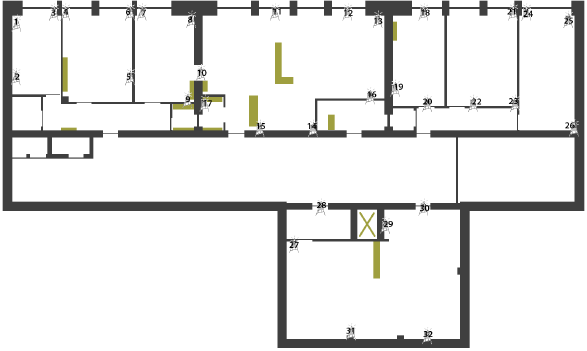
\includegraphics[scale=0.75]{content/images/Testbed}
   	\caption{Floor plan of the area where the Testbed is located. The position of the nodes is shown by the numbered antennas.}
    \label{fig:testbed}
\end{figure}

To monitor the area 32 nodes are distributed over the rooms like shown in Figure \ref{fig:testbed}. The nodes are only placed inside the offices and laboratories and are not always placed at the same hight. To make programming of the devices easy all the devices are connected to Raspberry Pies via USB. A script then makes it possible to copy the source code to all the Raspberry Pies where the code is compiled and then send to each node individual. The connection to the Raspberry Pies makes it also possible to collect information directly from each node individually over serial forwarder running on the Raspberry Pies.

\subsection{TelosB Mote}
The sensor nodes used for the Testbed are Crossbow's TelosB Motes TPR2420. The TPR2420 is a open source platform for researchers developed by the University of California, Berkley. It provides a 8 MHz Texas Instrument MSP430 low power microcontroller with 10kB RAM that is programmable via a USB connector. For communication it includes a IEEE 802.15.4 compliant radio frequency transceiver with an embedded antenna. This makes transmissions in a frequency band from 2.4 to 24835 GHz possible. Moreover the TPR2420 has a light sensor, a Infra-Red sensor, a humidity sensor and a temperature sensor installed making it possible to monitor the environment. Last it has three led lights installed that can be used for visual output of the mote. The USB connector that can be used to program the microcontroller can also be used to exchange data with and to power the TPR2420. If it is not connected via USB it can also be powered by two AA batteries. \cite{telosb}

\begin{figure}[htbp]
	\centering
    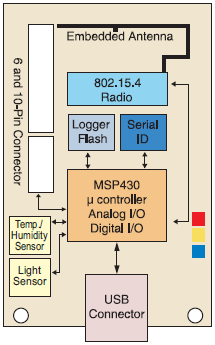
\includegraphics[scale=0.7]{content/images/Mote1}
   	\caption{The structure of the TPR2420 and the included components \cite{telosb}}
    \label{fig:telosb}
\end{figure}
 
\subsection{TinyOs}
TinyOS is an operating system for embedded systems, designed to manage the limited resources and power and to provide reactive concurrency and flexibility. It is widely used by multiple research groups ans companies world wide to support their applications.

The main tasks of TinyOS is to schedule tasks and events to provide safe concurrent operations. However it also provides a large amount of reusable system components, like timers, sender or receiver, that provide a huge variety of functionalities. When compiling a application only the TinyOS components that are used are included into the application creating an application-specific OS.

To provide functionality each component can have three different types of computational abstractions. First there are commands making it possible for other components to call a functionality of the component providing the command. Then there are events which can be signalled by a component. A component receiving the event can than react to it and act accordingly. These two constructs make interaction between components possible. For component intern functionality there are tasks. These can be posted by a component and then will be executed when its their turn. 

Whenever a command, event or task get called it is pushed into the queue of the TinyOS scheduler. The scheduler then executes the tasks inside the queue using a FIFO scheduling policy.    

\subsubsection{Programming for TinyOS}
Applications for TinyOS are written in nesC which us a C dialect and integrates the possibility to implement configurations, modules, interfaces, commands, Events and Tasks. An application consists of components, represented by a nesC module, that provide and use interfaces. The components implement the functionality of the application. All the commands and events a component provides are defined by an interface. Moreover an application for TinyOS also has a configuration that defines which components are connected.   

The Listings \ref{lis:Components}, \ref{lis:interface} and \ref{lis:configuration} show an example application for TinyOS with two components of which one provides an interface and the configuration for the application. This example shows the connections between components, interfaces and the configuration and also shows the use of commands, events and tasks. In Listing \ref{lis:Components} the two components $MainComponent$ and $ExampleC$ are represented. $MainComponent$ uses two interfaces. The first one is the $Boot$ interface. It requires the component to implement the $Boot.booted()$ event. This event is the first event signalled by TinyOS after the node booted. Moreover the $MainComponent$ uses the $ExampleI$ interface that is defined in Listing \ref{lis:interface}. It requires the component to implement the $ExampleI.exampleDone(error_t error)$. The $ExampleI$ interface is provided by the $ExampleC$ component and requires it to implement the $startExample()$ command. Moreover the $ExampleC$ component implements a task $doSomething()$.

Now to connect everything the configuration $Application$ in Listing \ref{lis:configuration} first calls all the components needed for the application. The first component used in this application is the $MainC$ component that provides the $Boot$ interface and is given by TinyOS. Next there are the two components from Listing \ref{lis:Components}. Know the configuration needs to connect the interfaces of the components to the components providing the corresponding interfaces. This means $MainComponent.Boot$ gets connected to $MainC$ and $MainComponent.ExampleI$ gets connected to $ExampleC$.

When a device would get programmed with this example the first thing that would happens is that $MainC$ signals $Boot.booted()$ event resulting in executing the code for the event inside $MainComponent$. This code calls the $ExampleI.startExample$ command. Since the interface is connected to the $ExampleC$ the corresponding code posting the $doSomething()$ task gets executed. Then at the end of $doSomething()$ the $ExampleI.exampleDone(...)$ gets signalled by $ExampleC$. This means the the event gets triggered in $MainComponent$ and the corresponding code gets executed.      

\lstset{caption={Two example components. $MainComponent$ uses the example interface from \ref{lis:interface} and the interface $Boot$ that TinyOS provides. $Boot$ requires the $MainComponent$ to implement the $Boot.booted()$ event that is the first event that gets signalled by TinyOS after the node booted. The $ExampleC$ provides the example interface and therefore needs to implement the event and also implements a task $doSomething()$.},label={lis:Components}}
\begin{lstlisting}
module MainComponent {
	uses interface Boot;
	uses interface ExampleI;
} implementation {
	event void Boot.booted() {
		call ExampleI.startExample();
	}
	
	event void ExampleI.exampleDone(error_t error) {
		if(error == SUCCESS) {
			//some task...
		}
	}
}

module ExampleC {
	provides interface ExampleI;
} implementation {
	task void doSomething() {
		//some task...
		
		signal ExampleI.exampleDone(SUCCESS);
	}
	
	command void startExample() {
		post doSomething();
	}
}
\end{lstlisting}


\lstset{caption={Example interface providing a command $startExample()$ and an event $exampleDone()$.},label={lis:interface}}
\begin{lstlisting}
interface ExampleI {
	command void startExample();
	event void exampleDone(error_t error);
}
\end{lstlisting}

\lstset{caption={The configuration $Application$ links all the Components},label={lis:configuration}}
\begin{lstlisting}
configuration Application {
} implementation {
	components MainC;
	components MainComponent
	components ExampleC;
		
	MainComponent.Boot -> MainC;
	MainComponent.ExampleI -> ExampleC;
}
\end{lstlisting} 

Since whenever a task, command or event gets called it does not get executed directly but gets added to the queue of the TinyOS scheduler. This means that all the tasks, commands or events called before will execute first including the currently running one. 